\documentclass[11pt]{article}

\usepackage{amsmath}
\usepackage{graphicx}

\title{Product Selection Optimization Under Budget Constraints}
\author{Esteban Murillo, Sebastian Lopez, Diego Bonilla}
\date{\today}

\begin{document}
\maketitle

\section{Polynomial-Time Reduction: Knapsack to Product Selection}

We reduce the classic \textbf{0--1 Knapsack Problem} (NP-hard) to our real-world problem, \textbf{Product Selection Under Budget Constraints}. In Knapsack, we are given items with \textbf{weights} and \textbf{values}, and a \textbf{capacity}; the goal is to select a subset of items of maximum total value without exceeding the capacity. In our setting, a store manager has products with \textbf{cost} (or shelf space used) and \textbf{promotional value} (or profit), plus a \textbf{budget} (or shelf-space limit); the goal is to maximize total promotional value without exceeding that limit.

\paragraph{How instances of the NP-hard problem are transformed.}
For each knapsack item, create one product. Table~\ref{tab:reduction} summarizes the correspondence. Concretely, a Knapsack instance with items $(w_i, v_i)$ and capacity $W$ becomes a product-selection instance with pairs $(\text{cost}_i, \text{value}_i)$ and budget $B$ by setting
\begin{equation*}
  \text{cost}_i = w_i,\qquad \text{value}_i = v_i,\qquad B = W.
\end{equation*}
The transformation copies each of the $n$ items once and renames fields, so it runs in $O(n)$ time and is polynomial.

\begin{table}[htbp]
  \centering
  \caption{Mapping from Knapsack to product selection.}
  \label{tab:reduction}
  \begin{tabular}{l l}
    \hline
    Knapsack problem & Product selection problem \\
    \hline
    Item & Product \\
    Weight & Cost or shelf-space used \\
    Value & Profit or promotional value \\
    Capacity & Budget or shelf-space limit \\
    \hline
  \end{tabular}
\end{table}

\paragraph{Why solving our problem implies a solution to the NP-hard problem.}
Suppose we had an algorithm that solves product selection optimally on every instance. Given any Knapsack instance, we construct the corresponding product-selection instance as above, run the algorithm, and interpret the chosen products as the chosen knapsack items. Because costs, values, and the budget match weights, values, and capacity pointwise, any feasible product subset corresponds to a feasible knapsack subset with the same total value, and optimality is preserved in both directions. Thus we could solve Knapsack in polynomial time (transformation plus one call to the product-selection solver). So product selection under budget constraints is at least as hard as Knapsack; since Knapsack is NP-hard, our problem is NP-hard as well.

\section{Test cases}

To evaluate the performance of the dynamic programming solution and heuristic or approximation algorithms, we tested it on five synthetic instances declared in our codebase as \texttt{datasets} in \texttt{datasets.py}. Each instance is a triple \texttt{(costs, values, budget)}: \texttt{costs} is \texttt{range(1, n+1)} and \texttt{values} is \texttt{range(10, 10n+1, 10)} for the corresponding number of products~$n$, with the budget~$B$ fixed as in the table. These instances match the tuples used when timing the bottom-up solver.

\begin{table}[htbp]
  \centering
  \caption{Experimental instances from \texttt{datasets.py} (costs and values are Python \texttt{range} objects as in the source file).}
  \label{tab:datasets}
  \begin{tabular}{r r r l l}
    \hline
    Case & $n$ & Budget $B$ & Costs (weights) $c_i$ & Values $v_i$ \\
    \hline
    1 & 5 & 20 & $1,2,\ldots,5$ & $10,20,\ldots,50$ \\
    2 & 10 & 50 & $1,2,\ldots,10$ & $10,20,\ldots,100$ \\
    3 & 20 & 100 & $1,2,\ldots,20$ & $10,20,\ldots,200$ \\
    4 & 30 & 200 & $1,2,\ldots,30$ & $10,20,\ldots,300$ \\
    5 & 50 & 300 & $1,2,\ldots,50$ & $10,20,\ldots,500$ \\
    \hline
  \end{tabular}
\end{table}

\section{Implementing an Algorithm that Guarantees an Optimal Solution}

We use the classical \textbf{bottom-up} dynamic program for the 0--1 knapsack. Let $n$ be the number of products (items) and let $W$ denote the budget (knapsack capacity). We build a table $\text{dp}[i][w]$ for $i \in \{0,\ldots,n\}$ and $w \in \{0,\ldots,W\}$, where $\text{dp}[i][w]$ is the maximum total promotional value achievable using only the first $i$ products and spending at most~$w$. Initially $\text{dp}[0][w]=0$ for all~$w$. For $i \ge 1$, letting $c_i$ be the cost (weight) and $v_i$ the value of product~$i$, we set
\begin{equation*}
  \text{dp}[i][w] =
  \begin{cases}
    \text{dp}[i-1][w], & c_i > w,\\[0.25em]
    \max\bigl(\text{dp}[i-1][w],\, v_i + \text{dp}[i-1][w-c_i]\bigr), & c_i \le w.
  \end{cases}
\end{equation*}
The optimal objective value is $\text{dp}[n][W]$. An optimal subset is recovered by \textbf{backtracking}: starting from $(i,w)=(n,W)$, if $\text{dp}[i][w] \neq \text{dp}[i-1][w]$ then product $i$ is taken and $w$ is reduced by~$c_i$; otherwise $i$ is skipped. This matches the order in which the table is filled (increasing $i$, then~$w$), so no recursion or memoization is needed---only a double loop over items and budget.

\paragraph{Time complexity.}
Each of the $n \cdot (W+1)$ states is computed in $O(1)$ time from earlier rows, and backtracking costs $O(n)$. Hence the running time is \textbf{$O(n \cdot W)$}, where $n$ is the number of items and $W$ is the capacity (budget). The table uses \textbf{$O(n \cdot W)$} space in the implementation we timed. Note that this is \emph{pseudopolynomial}: it depends on the numeric value of~$W$, not only on the bit-length of the input.

\subsection{Empirical timings}

We measured wall-clock time for the bottom-up implementation on each instance in Table~\ref{tab:datasets}. Figure~\ref{fig:dp_timing} plots the results. As $n$ and $W$ grow, the table has more rows and columns, so the observed time rises in line with filling an $(n+1)\times(W+1)$ grid---consistent with $O(n \cdot W)$. The growth is modest on these instances because $n\cdot W$ ranges from $100$ to $15{,}000$, but the curve is clearly non-decreasing as problem size increases.

\begin{figure}[htbp]
  \centering
  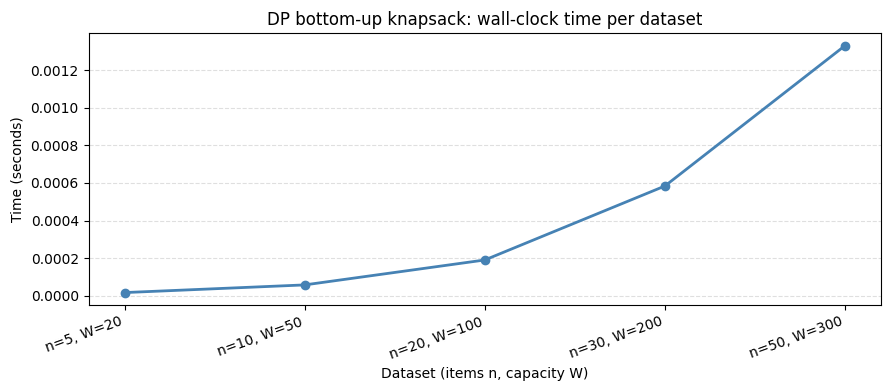
\includegraphics[width=0.95\textwidth]{photos/dp_bottomup_timing.png}
  \caption{Bottom-up dynamic programming: wall-clock time per dataset (labels show $n$ and capacity~$W$).}
  \label{fig:dp_timing}
\end{figure}


\end{document}
